\chapter{L'équilibre chimique~: quotient et constante}\label{ch:g12:equilibrium}

Une bouteille d'eau gazeuse fermée garde ses bulles pendant des mois~;
ouverte, elle est éventée en un après-midi. Rien d'anormal dans les deux
cas. Dans la bouteille fermée, le dioxyde de carbone quitte l'eau et y
revient à la même vitesse, et la composition ne bouge pas~; si l'on
ouvre le bouchon, le gaz qui s'en va ne revient plus. Beaucoup de
réactions se comportent ainsi~: elles s'arrêtent avant qu'aucun \omterm{def:g7:chemical-reactions:reactant}{réactif}
ne soit épuisé, sur un équilibre entre deux réactions opposées. Ce
chapitre décrit cet équilibre par un seul nombre.

\begin{recall}
L'\omterm{def:g10:reaction-progress-table:extent}{avancement} $x$ d'une réaction, son maximum $x_{\max}$, et les
\omterm{def:g10:reaction-progress-table:limiting}{réactions totales} qui l'atteignent (\cref{ch:g10:reaction-progress-table}).
La vitesse et les \omterm{def:g12:reaction-rates:kinetic-factor}{facteurs cinétiques} (\cref{ch:g12:reaction-rates})~; un
\omterm{def:g12:catalysis:catalyst}{catalyseur} ne modifie pas l'\omterm{def:g10:reaction-progress-table:system}{état final} (\cref{ch:g12:catalysis}).
\end{recall}

\begin{omfigure}
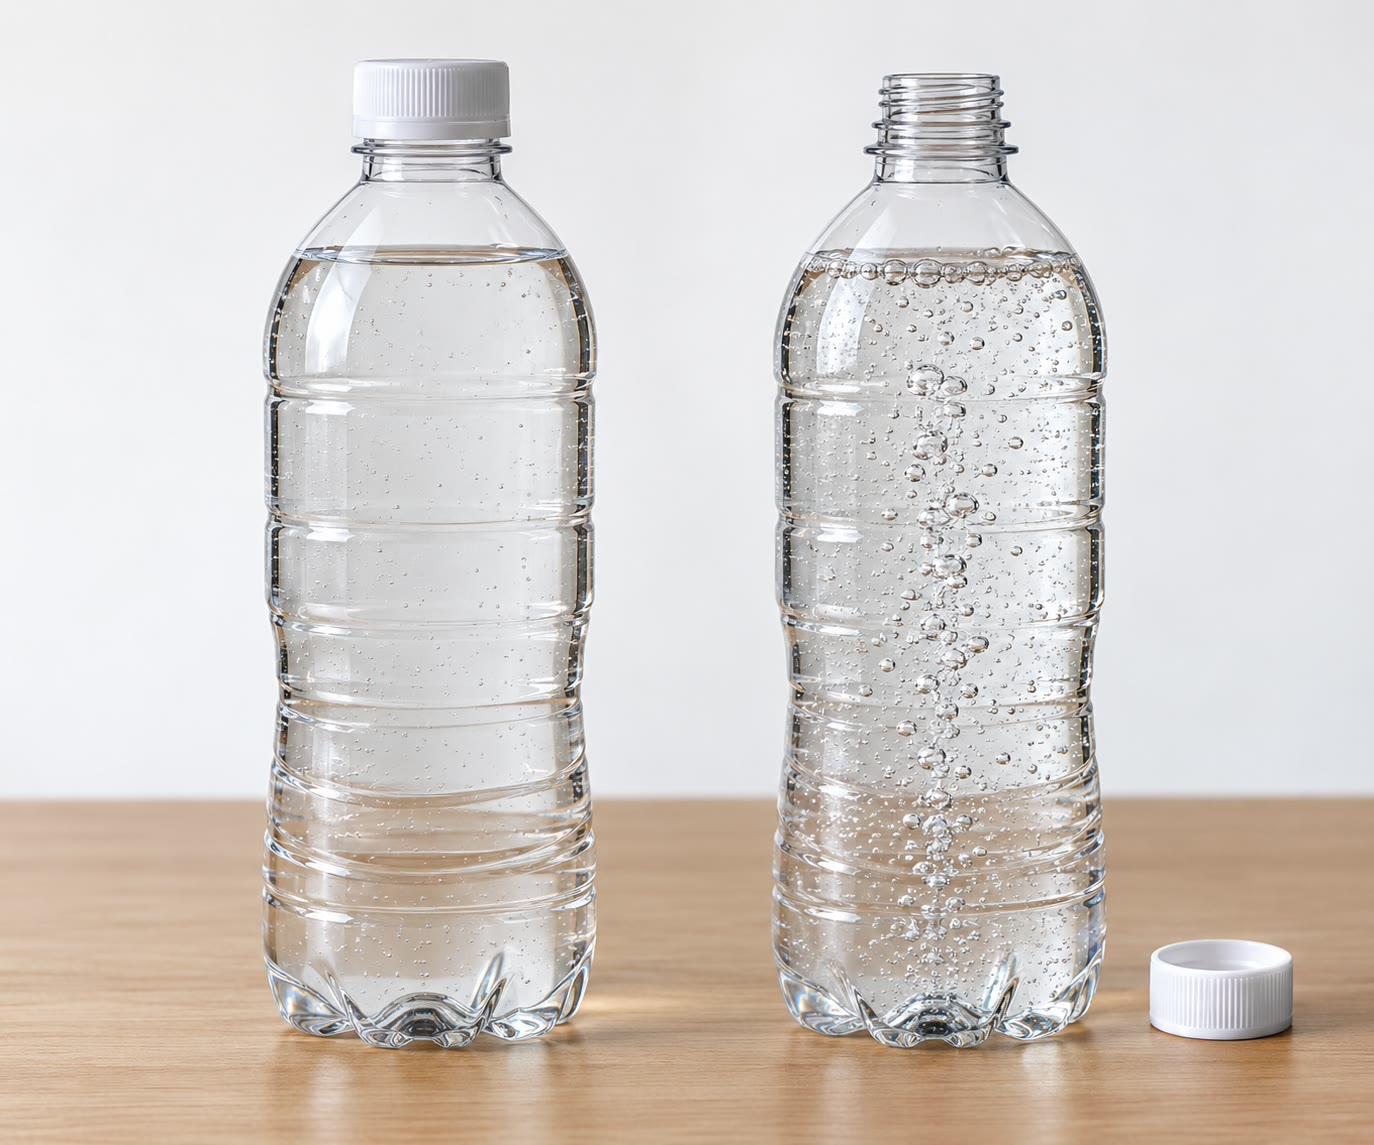
\includegraphics[width=0.45\linewidth,height=5cm,keepaspectratio]{images/book1/ai/g12-fizzy-bottles.jpg}

{\small Fermée, l'eau garde son gaz~; ouverte, le gaz s'échappe et ne
revient pas.}
\end{omfigure}

\section{Les réactions non totales}

\begin{definition}[Réaction non totale, taux d'avancement final]\label{def:g12:equilibrium:non-total}
Une réaction est une \emph{réaction non totale}\index{reaction non totale@réaction non totale}
si elle s'arrête à un \omterm{def:g10:reaction-progress-table:extent}{avancement} final $x_f$ inférieur à son \omterm{def:g10:reaction-progress-table:limiting}{avancement
maximal} $x_{\max}$, tous les \omterm{def:g7:chemical-reactions:reactant}{réactifs} étant encore présents. Son
\emph{taux d'avancement final}\index{taux d'avancement final} est
\[
  \tau = \frac{x_f}{x_{\max}}, \qquad 0 < \tau < 1
\]
($\tau = 1$ pour une \omterm{def:g10:reaction-progress-table:limiting}{réaction totale}).
\end{definition}

\begin{example}[Un ester qui s'arrête à mi-chemin]\label{ex:g12:equilibrium:berthelot}
% ledger: ester:berthelot
Chauffée avec \qty{1}{mol} d'éthanol, \qty{1}{mol} d'acide éthanoïque
forme de l'éthanoate d'éthyle et de l'eau,
\ce{CH3COOH + C2H5OH <=> CH3COOC2H5 + H2O}. La réaction s'arrête quand
environ les deux tiers de l'acide ont réagi~: $x_f = \qty{0.67}{mol}$
pour
$x_{\max} = \qty{1}{mol}$, donc $\tau \approx 0.67$. En partant de
\qty{1}{mol} d'\omterm{def:g11:functional-groups:carboxylic-acid}{ester} et de \qty{1}{mol} d'eau, la réaction inverse
s'arrête elle aussi, environ un tiers de l'\omterm{def:g11:functional-groups:carboxylic-acid}{ester} étant hydrolysé~: on
obtient le même \omterm{def:g6:pure-substances-and-mixtures:mixture}{mélange} final.
\end{example}

\begin{history}[Berthelot et Péan de Saint-Gilles, 1862]
% ledger: ester:berthelot
Les chimistes Marcellin Berthelot et Léon Péan de Saint-Gilles
chauffèrent longuement des \omterm{def:g6:pure-substances-and-mixtures:mixture}{mélanges} d'acide éthanoïque et d'éthanol, et
d'éthanoate d'éthyle et d'eau, puis les analysèrent. À partir de
quantités égales d'acide et d'\omterm{def:g11:functional-groups:alcohol}{alcool}, la réaction s'arrêtait toujours
vers les deux tiers~; à partir d'\omterm{def:g11:functional-groups:carboxylic-acid}{ester} et d'eau, à un tiers
d'hydrolyse~; et ils remarquèrent que la quantité d'\omterm{def:g11:functional-groups:carboxylic-acid}{ester} formée à
chaque instant dépendait du produit des quantités des \omterm{def:g7:chemical-reactions:reactant}{réactifs}. Leurs
travaux furent l'une des premières études quantitatives d'un équilibre
chimique.
\end{history}

\section{L'état d'équilibre}

\begin{definition}[État d'équilibre]\label{def:g12:equilibrium:equilibrium-state}
Un système est dans un \emph{état d'équilibre}\index{etat d'equilibre@état d'équilibre}
quand sa composition ne change plus alors que la réaction dans le sens
direct et la réaction dans le sens inverse se poursuivent toutes deux, à
la même vitesse. Une réaction qui peut atteindre un tel état s'écrit
avec la double flèche $\rightleftharpoons$.
\end{definition}

\begin{omfigure}
\begin{tikzpicture}
\begin{axis}[width=0.8\linewidth, height=6cm, xmin=0, xmax=200, ymin=0,
    ymax=1.05, xlabel={$t$ (\si{h})}, ylabel={quantité d'ester (\si{mol})},
    axis lines*=left, ymajorgrids, grid style={gray!20},
    tick label style={font=\small}, label style={font=\small},
    legend style={font=\small, at={(0.98,0.98)}, anchor=north east,
    draw=none, fill=white}, legend cell align=left]
  % ledger: ester:berthelot (K = 4; kinetics synthetic)
  \addplot[very thick, omDef] table[x=t, y=fromAcid] {figdata/out/grade-12-equilibrium.dat};
  \addplot[very thick, omProp] table[x=t, y=fromEster] {figdata/out/grade-12-equilibrium.dat};
  \addplot[dashed, black!60] coordinates {(0,0.6667) (200,0.6667)};
  \legend{acide + alcool (1 mol de chaque), ester + eau (1 mol de chaque)}
  \node[font=\small, anchor=north east] at (axis cs:195,0.65) {équilibre~: $\tfrac{2}{3}$ mol};
\end{axis}
\end{tikzpicture}

{\small L'estérification (en bleu) et l'hydrolyse de l'\omterm{def:g11:functional-groups:carboxylic-acid}{ester} (en orange)
atteignent la même composition d'équilibre, par des côtés opposés.
(L'échelle de temps est un modèle~; la valeur finale est la valeur
mesurée.)}
\end{omfigure}

\section{Le quotient de réaction}

\begin{notation}[Concentration standard]\label{not:g12:equilibrium:c-standard}
$c^\circ = \qty{1}{mol/L}$ est la concentration standard. Diviser une
concentration par $c^\circ$ donne un nombre sans unité de même
valeur~: $[\ce{A}]/c^\circ$.
\end{notation}

\begin{definition}[Quotient de réaction]\label{def:g12:equilibrium:quotient}
Pour une réaction en solution $a\,\ce{A} + b\,\ce{B} \rightleftharpoons c\,\ce{C} + d\,\ce{D}$, le \emph{quotient
de réaction}\index{quotient de reaction@quotient de réaction} dans un état donné du système
vaut
\[
  Q = \frac{\left([\ce{C}]/c^\circ\right)^c \left([\ce{D}]/c^\circ\right)^d}
           {\left([\ce{A}]/c^\circ\right)^a \left([\ce{B}]/c^\circ\right)^b} .
\]
Les solides, et le \omterm{def:g6:solutions-and-solubility:solute}{solvant} (l'eau dans une \omterm{def:g6:solutions-and-solubility:solute}{solution aqueuse}),
n'apparaissent pas dans
$Q$.
\end{definition}


\begin{example}[Écrire des quotients]\label{ex:g12:equilibrium:quotients}
Pour \ce{CH3COOH + H2O <=> CH3COO- + H3O+} dans l'eau (l'\omterm{def:g9:ions:ion}{ion} \ce{H3O+}
est présenté au chapitre suivant), l'eau est le \omterm{def:g6:solutions-and-solubility:solute}{solvant}~:
$Q = \dfrac{[\ce{CH3COO-}]\,[\ce{H3O+}]}{[\ce{CH3COOH}]\,c^\circ}$. Pour la
dissolution d'un solide, \ce{AgCl(s) <=> Ag+ + Cl-}, le solide est
omis~:
$Q = [\ce{Ag+}][\ce{Cl-}]/(c^\circ)^2$. Pour l'estérification, où les
quatre espèces sont dans le même \omterm{def:g6:pure-substances-and-mixtures:mixture}{mélange} liquide de volume $V$, les
volumes se simplifient et $Q = \dfrac{n_{\text{ester}}\, n_{\text{eau}}}{n_{\text{acide}}\, n_{\text{alcool}}}$.
\end{example}

\section{La constante d'équilibre}

\begin{definition}[Constante d'équilibre]\label{def:g12:equilibrium:constant}
La valeur $Q_{eq}$ du \omterm{def:g12:equilibrium:quotient}{quotient de réaction} dans l'\omterm{def:g12:equilibrium:equilibrium-state}{état d'équilibre} est
la \emph{constante d'équilibre}\index{constante d'equilibre@constante d'équilibre} $K$ de la
réaction. Elle est sans unité.
\end{definition}

\begin{proposition}[$K$ ne dépend que de la température]\label{prop:g12:equilibrium:constant}
Pour une réaction donnée, $Q_{eq} = K$ dans tout \omterm{def:g12:equilibrium:equilibrium-state}{état d'équilibre} à une
température donnée, quelles que soient les quantités initiales.
\end{proposition}

\begin{proof}
Admis~; cela est établi dans le volume de deuxième année d'université.
On le vérifie sur l'estérification~: les deux expériences de la figure,
parties de côtés opposés, donnent le même $Q_{eq}$.
\end{proof}

\begin{example}[La constante $K$ de l'estérification]\label{ex:g12:equilibrium:k-ester}
% ledger: ester:berthelot
À partir de \qty{1}{mol} d'acide et de \qty{1}{mol} d'\omterm{def:g11:functional-groups:alcohol}{alcool},
l'équilibre contient $\frac{2}{3}$ mol d'\omterm{def:g11:functional-groups:carboxylic-acid}{ester} et d'eau et
$\frac{1}{3}$ mol d'acide et d'\omterm{def:g11:functional-groups:alcohol}{alcool}~:
\[
  K = \frac{(2/3)\times(2/3)}{(1/3)\times(1/3)} = 4 .
\]
\end{example}

\begin{method}[État final d'une réaction non totale]\label{met:g12:equilibrium:final}
\begin{enumerate}
  \item Remplir le \omterm{def:g10:reaction-progress-table:extent}{tableau d'avancement} avec l'\omterm{def:g10:reaction-progress-table:extent}{avancement} final inconnu
        $x_f$.
  \item Écrire $Q_{eq}$ en fonction de $x_f$ et l'égaler à $K$.
  \item Résoudre en $x_f$ (c'est souvent une équation du second degré),
        en gardant la racine comprise entre 0 et $x_{\max}$.
  \item En déduire les quantités finales et $\tau = x_f/x_{\max}$.
\end{enumerate}
\end{method}

\begin{example}[Un excès d'alcool]\label{ex:g12:equilibrium:excess}
À partir de \qty{1}{mol} d'acide et de \qty{2}{mol} d'\omterm{def:g11:functional-groups:alcohol}{alcool}~:
$\dfrac{x^2}{(1-x)(2-x)} = 4$, soit $3x^2 - 12x + 8 = 0$, dont la racine
comprise entre 0 et 1 est $x_f = \qty{0.845}{mol}$. Doubler la quantité
d'\omterm{def:g11:functional-groups:alcohol}{alcool} fait passer le \omterm{def:g10:synthesis-yield:yield}{rendement}, calculé par rapport à l'acide, de
\qty{67}{\percent} à
\qty{85}{\percent}.
\end{example}

\section{Prévoir et déplacer l'évolution}

\begin{proposition}[Sens d'évolution]\label{prop:g12:equilibrium:direction}
Si $Q < K$, le système évolue dans le sens direct (les produits
augmentent) jusqu'à ce que $Q = K$~; si $Q > K$, il évolue dans le sens
inverse~;
si $Q = K$, il est à l'équilibre et n'évolue pas.
\end{proposition}

\begin{proof}
Admis~: $Q$ augmente quand la réaction progresse dans le sens direct
(les produits, au numérateur, augmentent, et les \omterm{def:g7:chemical-reactions:reactant}{réactifs}, au
dénominateur, diminuent), et le système évolue vers l'état où $Q = K$.
\end{proof}

\begin{omfigure}
\begin{tikzpicture}[font=\small]
  \draw[->, thick] (0,0) -- (10,0) node[right] {$Q$};
  \draw[thick] (0,-0.12) -- (0,0.12) node[above] {0};
  \draw[very thick, omThm] (5,-0.25) -- (5,0.25) node[above] {$K$};
  \draw[->, very thick, omDef] (1.2,0.55) -- (4.4,0.55);
  \node[omDef, align=center] at (2.8,1.15) {$Q < K$~: sens direct};
  \draw[->, very thick, omProp] (8.8,0.55) -- (5.6,0.55);
  \node[omProp, align=center] at (7.2,1.15) {$Q > K$~: sens inverse};
  \node[align=center] at (5,-0.75) {$Q = K$~: équilibre};
\end{tikzpicture}

{\small Le quotient évolue toujours vers la constante.}
\end{omfigure}

\begin{remark}[Déplacer un équilibre]\label{rem:g12:equilibrium:shift}
Pour obtenir davantage de produit d'une \omterm{def:g12:equilibrium:non-total}{réaction non totale}, on peut
mettre un \omterm{def:g7:chemical-reactions:reactant}{réactif} en excès (le moins cher), ou éliminer un produit au
fur et à mesure qu'il se forme~: dans les deux cas, $Q < K$ de nouveau,
et le système évolue dans le sens direct. Éliminer l'eau d'une
estérification (par un desséchant, ou en la distillant) peut rendre la
réaction presque totale. La bouteille d'eau gazeuse ouverte fait de même
avec le dioxyde de carbone qui s'échappe.
\end{remark}

\begin{omfigure}
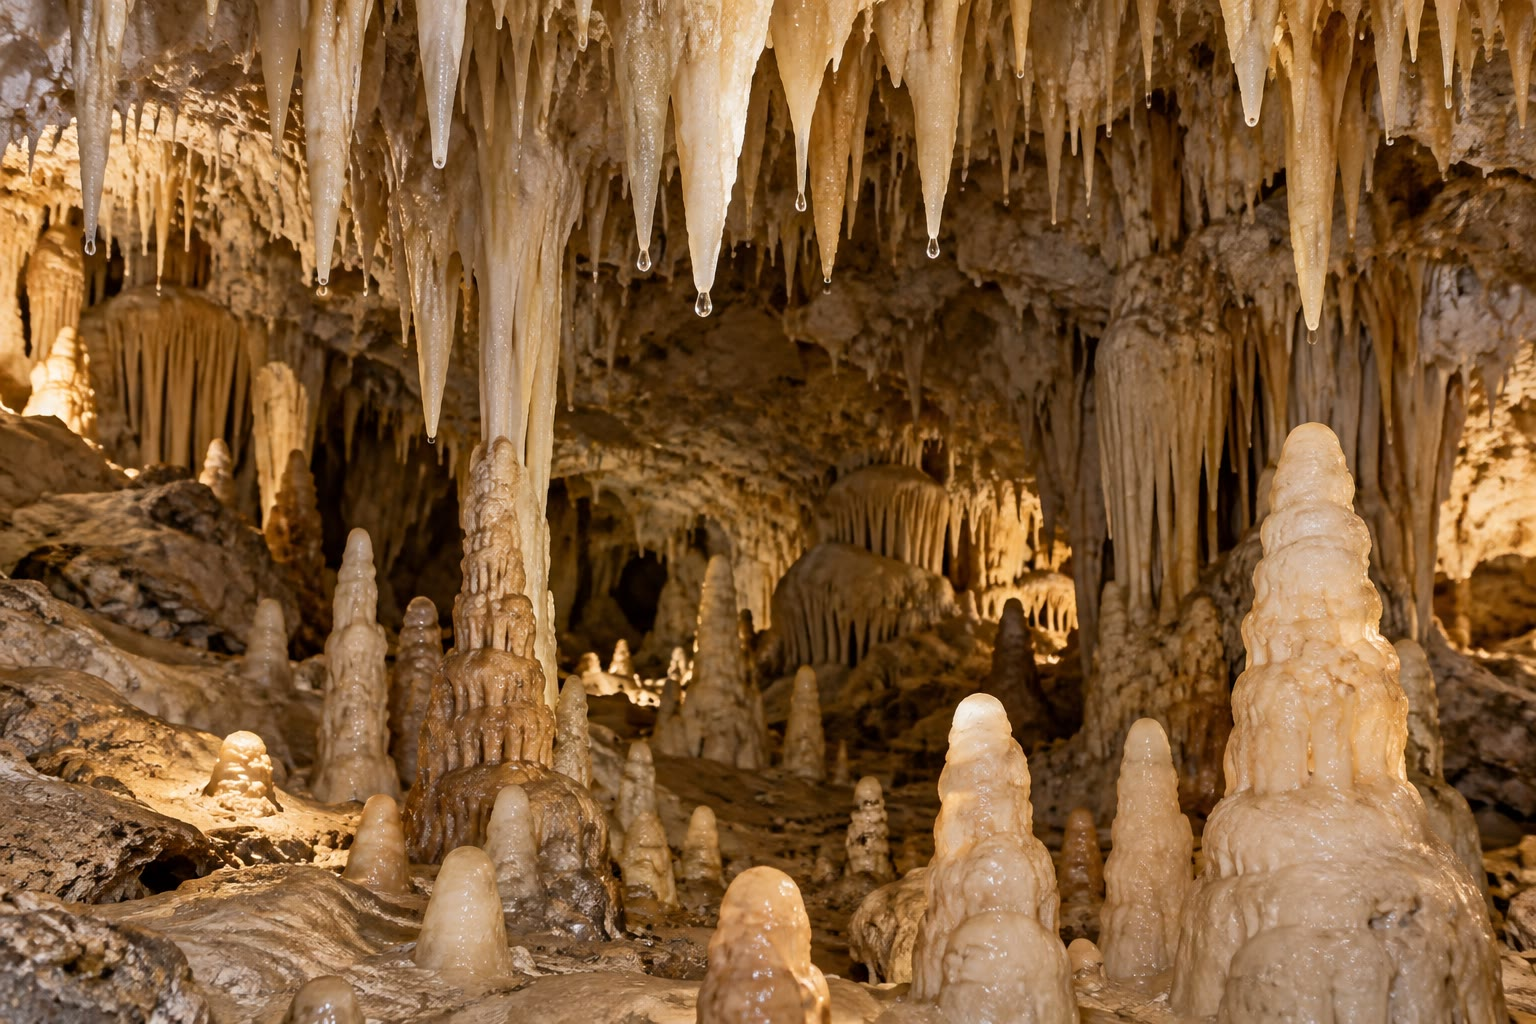
\includegraphics[width=0.45\linewidth]{images/book1/ai/g12-cave-stalactites.jpg}

{\small Les stalactites croissent là où l'eau qui goutte dans une grotte
cède du dioxyde de carbone à l'\omterm{def:g4:air-a-mixture-of-gases:air}{air}~: un équilibre de dissolution du
calcaire est déplacé, et du carbonate de calcium se dépose.}
\end{omfigure}

\section{Exercices}

\begin{exercise}[$\star$]\label{exo:g12:equilibrium:1}
Écrire le \omterm{def:g12:equilibrium:quotient}{quotient de réaction} de~: (a) \ce{N2 + 3H2 <=> 2NH3} (gaz~;
utiliser les concentrations)~; (b) \ce{CH3COOH + H2O <=> CH3COO- + H3O+}
dans l'eau~;
(c) \ce{CaCO3(s) <=> Ca^{2+} + CO3^{2-}}~; (d) \ce{Fe^{3+} + SCN- <=>
FeSCN^{2+}}.
\end{exercise}

\begin{exercise}[$\star$]\label{exo:g12:equilibrium:2}
Une réaction a pour $x_{\max} = \qty{0.050}{mol}$ et atteint
$x_f = \qty{0.020}{mol}$. Calculer $\tau$. La réaction est-elle
totale~?
\end{exercise}

\begin{exercise}[$\star$]\label{exo:g12:equilibrium:3}
Pour une réaction de constante $K = 10$, dans quel sens évolue un
\omterm{def:g6:pure-substances-and-mixtures:mixture}{mélange} si
$Q = 2$~? Si $Q = 50$~? Si $Q = 10$~?
\end{exercise}

\begin{exercise}[$\star$]\label{exo:g12:equilibrium:4}
Expliquer pourquoi on dit d'un équilibre qu'il est «~dynamique~».
\end{exercise}

\begin{exercise}[$\star$]\label{exo:g12:equilibrium:5}
Un \omterm{def:g12:catalysis:catalyst}{catalyseur} modifie-t-il $K$~? La durée nécessaire pour atteindre
l'équilibre~? Expliquer.
\end{exercise}

\begin{exercise}[$\star\star$]\label{exo:g12:equilibrium:6}
On \omterm{def:g6:pure-substances-and-mixtures:mixture}{mélange} \qty{2.0}{mol} d'acide éthanoïque et \qty{2.0}{mol}
d'éthanol ($K = 4$). Calculer les quantités finales des quatre espèces.
\end{exercise}

\begin{exercise}[$\star\star$]\label{exo:g12:equilibrium:7}
Un \omterm{def:g6:pure-substances-and-mixtures:mixture}{mélange} contient \qty{0.5}{mol} de chacune des espèces suivantes~:
acide éthanoïque, éthanol, éthanoate d'éthyle et eau. Calculer $Q$. Dans
quel sens évolue-t-il~?
\end{exercise}

\begin{exercise}[$\star\star$]\label{exo:g12:equilibrium:8}
À l'aide de la figure des deux expériences, lire la quantité d'\omterm{def:g11:functional-groups:carboxylic-acid}{ester}
au bout de
\qty{20}{h} dans chacune. À partir de quand peut-on considérer que le
système est à l'équilibre~?
\end{exercise}

\begin{exercise}[$\star\star$]\label{exo:g12:equilibrium:9}
En partant de \qty{1}{mol} d'\omterm{def:g11:functional-groups:carboxylic-acid}{ester} et de \qty{1}{mol} d'eau ($K = 4$
pour l'estérification, donc $1/4$ pour l'hydrolyse), calculer les
quantités finales par la méthode du chapitre, et comparer avec
l'expérience d'estérification.
\end{exercise}

\begin{exercise}[$\star\star$]\label{exo:g12:equilibrium:10}
Pourquoi le solide n'apparaît-il pas dans le quotient de
\ce{AgCl(s) <=> Ag+ + Cl-}~? Ajouter du solide déplace-t-il
l'équilibre~?
\end{exercise}

\begin{exercise}[$\star\star$]\label{exo:g12:equilibrium:11}
Dans une bouteille d'eau gazeuse fermée, le dioxyde de carbone quitte
l'eau et y entre à la même vitesse. Écrire l'équilibre
\ce{CO2(aq) <=> CO2(g)} et expliquer, à l'aide de $Q$ et de $K$,
pourquoi l'eau s'évente quand on ouvre la bouteille.
\end{exercise}

\begin{exercise}[$\star\star\star$]\label{exo:g12:equilibrium:12}
Une estérification de \qty{1}{mol} d'acide et de \qty{1}{mol} d'\omterm{def:g11:functional-groups:alcohol}{alcool}
atteint l'équilibre. On retire alors la moitié de l'eau présente.
Calculer le nouveau $Q$, dire dans quel sens le système évolue, et
trouver la nouvelle quantité finale d'\omterm{def:g11:functional-groups:carboxylic-acid}{ester}.
\end{exercise}

\begin{exercise}[$\star\star\star$]\label{exo:g12:equilibrium:13}
Montrer que la constante de la réaction inverse vaut $1/K$. Quelle est
la constante de l'hydrolyse de l'éthanoate d'éthyle~?
\end{exercise}

\begin{exercise}[$\star\star\star$]\label{exo:g12:equilibrium:14}
Un chimiste \omterm{def:g6:pure-substances-and-mixtures:mixture}{mélange} \qty{1}{mol} d'acide, \qty{1}{mol} d'\omterm{def:g11:functional-groups:alcohol}{alcool},
\qty{2}{mol} d'\omterm{def:g11:functional-groups:carboxylic-acid}{ester} et \qty{0.5}{mol} d'eau. Va-t-il se passer quelque
chose~? Expliquer.
\end{exercise}

\begin{exercise}[$\star\star\star$]\label{exo:g12:equilibrium:15}
Quel excès d'\omterm{def:g11:functional-groups:alcohol}{alcool} (quantité par \omterm{def:g10:the-mole:amount}{mole} d'acide) faut-il pour estérifier
\qty{95}{\percent} de l'acide~? Résoudre $\dfrac{0.95^2}{0.05(n - 0.95)} =
4$.
\end{exercise}

\section{Problème~: l'ester de Berthelot}

\begin{problem}[{Problème du week-end --- quelle quantité d'ester quand
l'alcool est mis en excès d'un facteur trois~?}]
\label{pb:g12:equilibrium:1}
% ledger: ester:berthelot, aw:C, aw:H, aw:O
L'éthanoate d'éthyle, un \omterm{def:g6:solutions-and-solubility:solute}{solvant} et un arôme, se prépare à partir
d'acide éthanoïque et d'éthanol. En 1862, Berthelot et Péan de
Saint-Gilles trouvèrent qu'à partir de quantités égales d'acide et
d'\omterm{def:g11:functional-groups:alcohol}{alcool}, la réaction s'arrête quand environ les deux tiers de l'acide
ont réagi.

\medskip
\noindent\textbf{Partie I --- La réaction.}
\begin{enumerate}
  \item Écrire l'équation de l'estérification, avec des \omterm{def:g11:organic-skeletons:formulas}{formules
        semi-développées}.
  \item Pourquoi l'écrit-on avec une double flèche~?
  \item Écrire son \omterm{def:g12:equilibrium:quotient}{quotient de réaction} en \omterm{def:g10:the-mole:amount}{quantités de matière}.
  \item À partir de \qty{1}{mol} d'acide et de \qty{1}{mol} d'\omterm{def:g11:functional-groups:alcohol}{alcool},
        que vaut $x_{\max}$~? Que vaut $x_f$, d'après le résultat de
        Berthelot~?
  \item Calculer $\tau$.
\end{enumerate}

\medskip
\noindent\textbf{Partie II --- La constante.}
\begin{enumerate}[resume]
  \item Donner les quantités finales des quatre espèces.
  \item Calculer $K$.
  \item En partant de \qty{1}{mol} d'\omterm{def:g11:functional-groups:carboxylic-acid}{ester} et de \qty{1}{mol} d'eau,
        Berthelot trouva un tiers d'\omterm{def:g11:functional-groups:carboxylic-acid}{ester} hydrolysé. Montrer que ce
        résultat est en accord avec la même constante $K$.
  \item Pourquoi $K$ doit-elle être la même dans les deux cas~?
\end{enumerate}

\medskip
\noindent\textbf{Partie III --- Un excès d'\omterm{def:g11:functional-groups:alcohol}{alcool} d'un facteur trois.}
\begin{enumerate}[resume]
  \item À partir de \qty{1}{mol} d'acide et de \qty{3}{mol} d'\omterm{def:g11:functional-groups:alcohol}{alcool},
        remplir le \omterm{def:g10:reaction-progress-table:extent}{tableau d'avancement}.
  \item Écrire l'équation $Q_{eq} = K$ et montrer qu'elle devient
        $3x^2 - 16x + 12 = 0$.
  \item La résoudre, et garder la racine qui a un sens.
  \item Quelle fraction de l'acide est estérifiée~?
  \item Calculer la masse d'\omterm{def:g11:functional-groups:carboxylic-acid}{ester} obtenue.
\end{enumerate}

\medskip
\noindent\textbf{Partie IV --- Éliminer l'eau.}
\begin{enumerate}[resume]
  \item À partir de l'équilibre obtenu avec un \omterm{def:g6:pure-substances-and-mixtures:mixture}{mélange} équimolaire, on
        élimine l'eau au fur et à mesure qu'elle se forme. Expliquer à
        l'aide de $Q$ pourquoi la réaction se poursuit.
  \item Si toute l'eau pouvait être éliminée, que deviendrait le
        \omterm{def:g10:synthesis-yield:yield}{rendement}~?
  \item Pourquoi met-on d'habitude l'\omterm{def:g11:functional-groups:alcohol}{alcool}, et non l'acide, en excès~?
        (Penser au coût et à la séparation des produits.)
  \item Chauffer le \omterm{def:g6:pure-substances-and-mixtures:mixture}{mélange} modifie-t-il l'\omterm{def:g10:reaction-progress-table:system}{état final}, ou seulement la
        durée nécessaire pour l'atteindre~? (L'estérification ne dégage
        presque pas de chaleur.)
  \item Donner la réponse finale~: quelle fraction de l'acide est
        estérifiée avec un excès d'\omterm{def:g11:functional-groups:alcohol}{alcool} d'un facteur trois~?
\end{enumerate}
\end{problem}
